
\documentclass[12pt]{article}

\usepackage[margin=1in]{geometry}
\usepackage{setspace}
\usepackage{booktabs}
\usepackage{graphicx}
\usepackage{amsmath, amssymb}
\usepackage{natbib}
\usepackage{hyperref}
\usepackage{longtable}
\usepackage{array}

\onehalfspacing
\bibliographystyle{aer}

\title{\Large{Why might the quality of goods sold be extremely poor?}\\\large{\textit{An Agent-Based Interpretation of Steinbeck's Market for Jalopies}}}
\author{ChatGPT (OpenAI, GPT-5.3)}

\date{\today}

\begin{document}

\maketitle

\begin{abstract}
This paper develops an agent-based interpretation of the market for used cars described in John Steinbeck's \textit{The Grapes of Wrath}. The point of departure is the standard lemons mechanism associated with \citet{akerlof1970}, in which asymmetric information about quality can drive high-quality goods out of the market. The central argument of the paper, however, is that the Steinbeck case is not adequately captured by asymmetric information alone. In the environment described by Steinbeck, buyers are under severe pressure to purchase immediately, possess little knowledge not only of quality but also of market tactics, confront locally powerful sellers in one-shot interactions, and enjoy little effective institutional protection. The paper formalizes this richer interpretation through an agent-based model in which urgency, low market literacy, vulnerability-sensitive price discrimination, seller opportunism, and weak institutions interact with imperfect information. The model generates persistent low-quality equilibria even when the market does not collapse completely. In this sense, the Steinbeck market is interpreted not as a mere literary illustration of the Akerlof problem, but as a distinct and recurrent configuration of distressed exchange.
\end{abstract}

\section{Introduction}

The used-car market described in Chapter 7 of \textit{The Grapes of Wrath} is one of the sharpest literary depictions of predatory exchange under crisis conditions. Families forced off the land must liquidate what they own, purchase transportation quickly, and embark upon a migration whose success depends on a machine they are poorly positioned to evaluate. Sellers, by contrast, are portrayed as organized, fast, locally dominant, and acutely aware of how to exploit vulnerability. In this environment, market exchange is neither anonymous nor frictionless. It is structured by asymmetries of information, urgency, bargaining weakness, and the practical absence of corrective institutions.

A natural theoretical reference point is \citet{akerlof1970}. In Akerlof's canonical account, quality heterogeneity and asymmetric information suffice to explain why low-quality goods can dominate a market. Buyers discount their offers because they cannot distinguish good cars from bad ones; sellers of high-quality goods withdraw; the average quality of market supply deteriorates. This mechanism is central to any interpretation of the Steinbeck episode. Yet it is not sufficient.

The Steinbeck market contains additional elements that matter analytically. First, demand is constrained not in the sense of a standard shift in preferences, but in the sense that purchase is urgent and cannot easily be postponed. Second, buyers are weakly informed not only about product quality, but also about the routines, scripts, and traps of the market itself. Third, the market has a one-shot character: sellers do not need to preserve a durable reputation with a stable clientele. Fourth, pricing is not merely an average response to uncertainty; it is actively tailored to perceived vulnerability. Fifth, institutions capable of imposing minimum quality standards or credible redress are weak or absent.

This paper develops these ideas in the form of a transparent agent-based model. The objective is not to calibrate the model tightly to a single historical dataset, but rather to construct a disciplined theoretical laboratory capable of separating mechanisms. The model distinguishes a relatively pure lemons environment from an extended Steinbeck environment in which informational asymmetry is reinforced by forced demand, socio-anthropological vulnerability, opportunistic pricing, and weak institutional constraints. The key result is that persistent low-quality equilibria can arise and remain profitable even without complete market shutdown.

\section{Literature and conceptual background}

The standard theoretical benchmark is \citet{akerlof1970}, whose account of quality uncertainty remains foundational. In that framework, the deterioration of average quality is driven by the interaction of hidden information and heterogeneous goods. The broader implication is that certain markets may become thin or fail altogether.

The Steinbeck episode invites a broader reading. It is a market in which social position, crisis, migration, and institutional weakness jointly shape exchange. The historical and literary context of the Great Depression has been emphasized by \citet{dickstein2004} and \citet{dyen2010}. The symbolic and class dimensions of automobiles in Steinbeck have been examined by \citet{delucia2014}. The present paper is complementary to those contributions: it translates the textual and historical intuition into a formal computational framework.

The central conceptual distinction is between a pure informational market failure and a distressed-exchange market failure. In the former, the problem is that buyers do not observe quality. In the latter, buyers also face urgency, low market literacy, and structural bargaining weakness. This second configuration is not universal in the same abstract sense as the Akerlof benchmark. Yet it is historically recurrent. Migration waves, displacement crises, and markets serving transient and vulnerable populations repeatedly generate exchange environments in which sellers can profit more from low quality than from durability.

\section{Model}

\subsection{Agents, goods, and time}

Time is discrete, and one period corresponds to one week. In each week, a flow of buyers enters the market and meets a population of sellers. Sellers hold inventories of used cars. Each car has a true quality $q \in [0,1]$, a seller cost $c$, and a quality label indicating whether it is a lemon.

Each buyer has a budget $B_i$, urgency $u_i$, market literacy $\ell_i$, and risk tolerance $r_i$. A synthetic vulnerability index $v_i$ combines high urgency and low literacy. Intuitively, a buyer with urgent transport needs and poor understanding of market practices is easier to exploit.

\subsection{Quality perception and reservation value}

Buyer $i$ does not observe true quality directly. Instead, the buyer forms a perceived quality
\begin{equation}
\tilde q_i = \min\{1, \max\{0, q + \varepsilon_i\}\},
\end{equation}
where $\varepsilon_i$ is a noise term whose variance rises with informational asymmetry and falls with market literacy.

The buyer's reservation price is increasing in perceived quality, urgency, and risk tolerance:
\begin{equation}
R_i = B_i \, \tilde q_i \, (1 + \alpha u_i)(1 + \beta r_i).
\end{equation}
A buyer purchases if the quoted price is sufficiently low relative to this reservation value, or, in very high-urgency states, if the offer remains within the budget constraint. This rule captures the idea that desperation can override strict screening.

\subsection{Seller pricing}

Seller pricing is based on cost, but it also depends on the buyer's vulnerability and on the scope for opportunism:
\begin{equation}
P_{ij} = c_j (1+m)\left[(1 + \delta v_i) + \gamma L_j \right](1-\kappa),
\end{equation}
where $m$ is the base markup, $\delta$ captures vulnerability-based price discrimination, $\gamma$ captures opportunism, $L_j$ is an indicator for a lemon, and $\kappa$ is a competition effect that reduces effective overcharging power. The model therefore allows low-quality cars to become especially profitable under the right conditions.

\subsection{Institutions}

Institutions operate through simple inspections and quality screening. With probability increasing in institutional strength, a trade is inspected. Very low-quality cars can be removed from the market, and inspected lemon sales yield lower net revenue for the seller through a fine-like mechanism. This captures, in compressed form, the effects of quality standards, inspections, and legal risk.

\section{Simulation design}

The notebook associated with this paper runs weekly simulations and compares alternative market regimes. The central scenarios are:

\begin{enumerate}
    \item an \textit{Akerlof-like} scenario with quality uncertainty but weaker Steinbeck amplification;
    \item a \textit{Steinbeck distressed market} with high urgency, low literacy, stronger opportunism, and limited institutional correction;
    \item an \textit{institutional correction} scenario in which screening is strengthened;
    \item a \textit{more competitive} scenario in which effective seller power is reduced.
\end{enumerate}

The notebook saves both figures and tables directly into the package directories \texttt{figures/} and \texttt{tables/}. The LaTeX source below is written to include those outputs after the notebook has been run.

\section{Results and interpretation}

The model is designed to generate several qualitative propositions.

First, in a relatively pure lemons environment, informational asymmetry alone can raise the share of low-quality cars sold. However, when urgency is modest and literacy is relatively high, average quality need not collapse dramatically.

Second, once urgency rises and literacy falls, seller pricing becomes more exploitative and the relative profitability of lemons increases. This is the distinctly Steinbeckian mechanism. The market need not disappear; instead, it can survive precisely because vulnerable buyers continue purchasing.

Third, stronger institutions can lower lemon prevalence by directly removing the worst cars and by reducing the expected revenue from exploitative sales. Likewise, stronger competition can diminish the pricing power that sellers exercise over desperate buyers.

If the notebook has been run, the following outputs will be available.

\begin{figure}[h!]
\centering
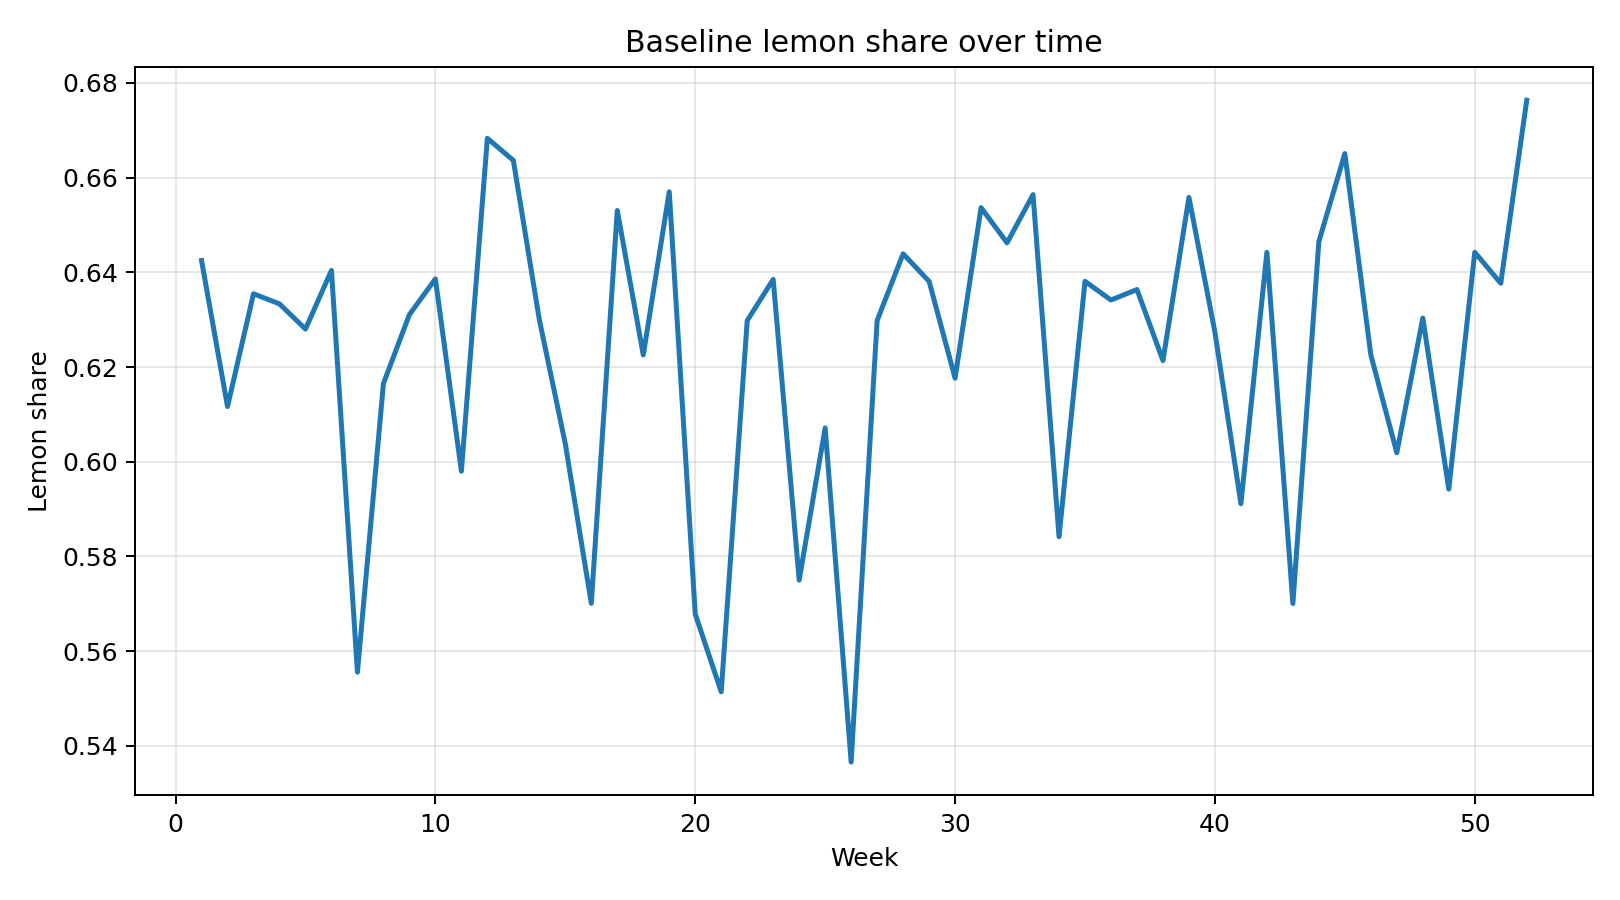
\includegraphics[width=0.75\textwidth]{figures/baseline_lemon_share.png}
\caption{Baseline weekly lemon share.}
\label{fig:baseline_lemon_share}
\end{figure}

\begin{figure}[h!]
\centering
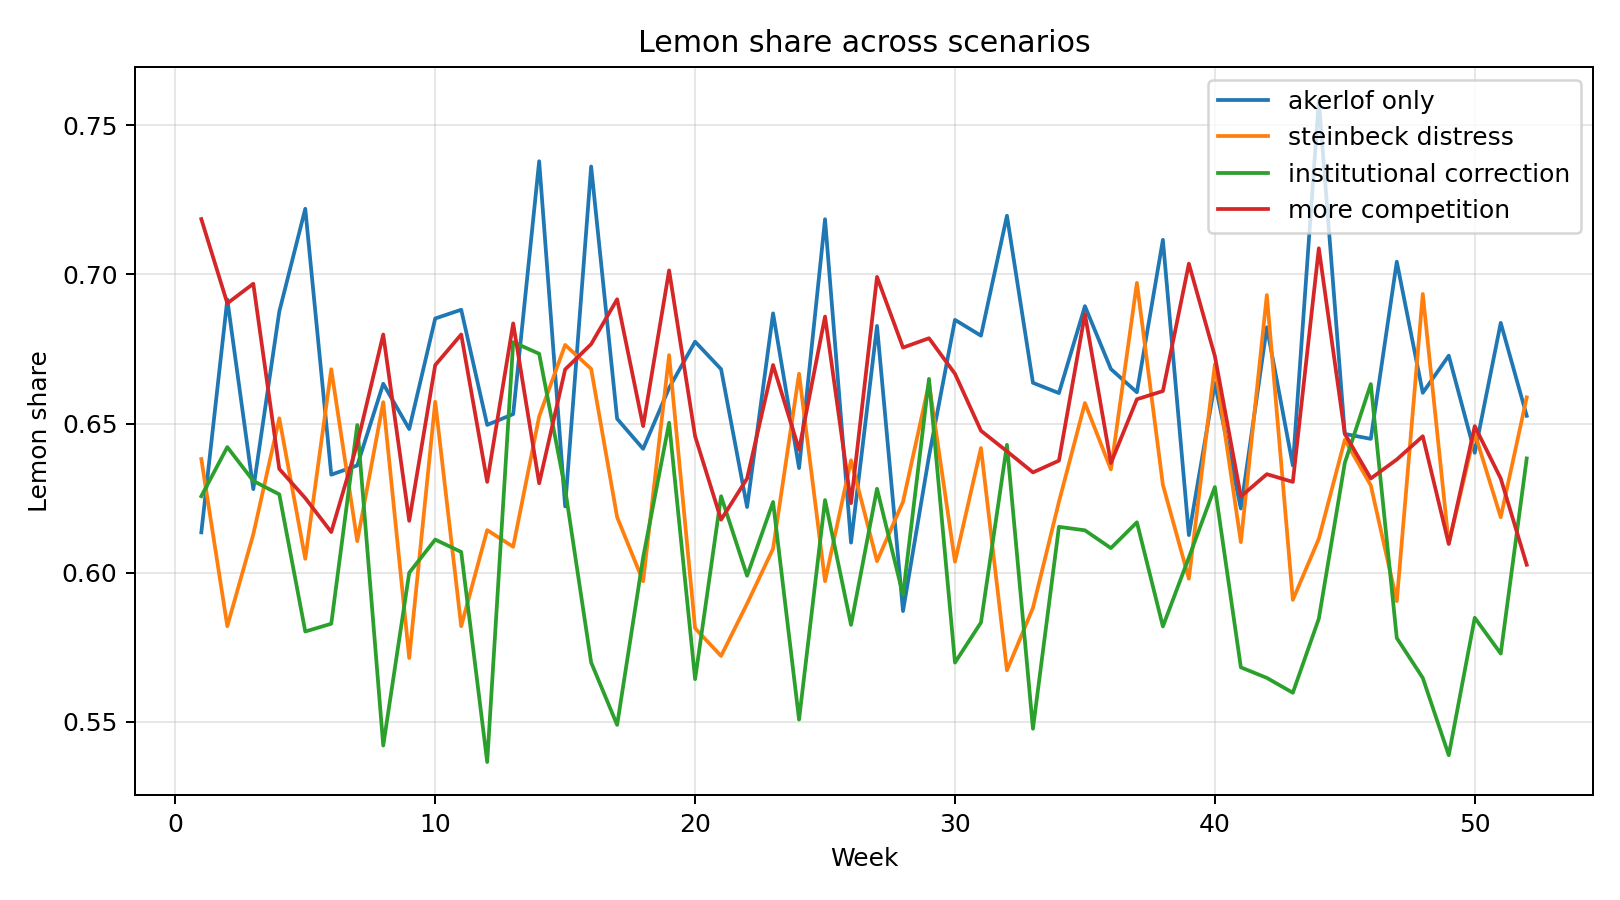
\includegraphics[width=0.75\textwidth]{figures/scenario_comparison_lemon_share.png}
\caption{Lemon share across stylized scenarios.}
\label{fig:scenario_comparison_lemon_share}
\end{figure}

\begin{table}
\caption{Summary statistics for the baseline scenario.}
\label{tab:baseline_summary}
\begin{tabular}{lrrrrrrrrr}
\toprule
scenario & weeks & total\_trades & mean\_weekly\_trades & mean\_lemon\_share & mean\_avg\_quality & mean\_avg\_price & mean\_buyer\_surplus & mean\_seller\_revenue & blocked\_sales\_total \\
\midrule
baseline & 52 & 10728 & 206.307700 & 0.623300 & 0.480100 & 101.677500 & 58.807000 & 101.346600 & 173 \\
\bottomrule
\end{tabular}
\end{table}


\begin{table}
\caption{Comparison of stylized scenarios.}
\label{tab:scenario_comparison_summary}
\begin{tabular}{lrrrrrrrrr}
\toprule
scenario & weeks & total\_trades & mean\_weekly\_trades & mean\_lemon\_share & mean\_avg\_quality & mean\_avg\_price & mean\_buyer\_surplus & mean\_seller\_revenue & blocked\_sales\_total \\
\midrule
akerlof\_only & 52 & 11020 & 211.923100 & 0.665300 & 0.456700 & 62.631900 & 58.054800 & 62.417800 & 186 \\
steinbeck\_distress & 52 & 10806 & 207.807700 & 0.626900 & 0.478100 & 121.800600 & 54.910600 & 121.692200 & 107 \\
institutional\_correction & 52 & 10182 & 195.807700 & 0.602200 & 0.499100 & 124.973700 & 54.146000 & 114.628200 & 786 \\
more\_competition & 52 & 11859 & 228.057700 & 0.655100 & 0.459700 & 75.175200 & 67.088700 & 75.108100 & 140 \\
\bottomrule
\end{tabular}
\end{table}


\section{Why the Steinbeck case is not simply Akerlof}

The model clarifies why the Steinbeck market should not be interpreted as a literary restatement of the canonical lemons story. Akerlof's mechanism is about hidden quality and adverse selection. The Steinbeck case certainly contains that element, but it also includes a second mechanism: the active monetization of vulnerability.

A buyer in Steinbeck's environment is not merely uncertain; the buyer is pressed by necessity, weakly informed about transactional practice, and placed in a one-shot exchange with little possibility of recourse. These conditions enable a seller to earn more on low-quality goods than on durable ones. That is why an excess of demand alone does not explain the outcome. Excess demand can raise prices temporarily. It does not, by itself, explain why sellers should prefer to circulate especially poor goods. The answer lies in the conjunction of informational asymmetry, vulnerability-sensitive extraction, and weak institutions.

\section{Conclusion}

The paper has proposed an agent-based interpretation of Steinbeck's used-car market that preserves the insights of Akerlof while moving beyond them. The contribution is conceptual rather than narrowly empirical. The model demonstrates how a market can remain active, and even lucrative for sellers, while systematically channeling bad goods to vulnerable buyers. This is not a universal market structure, but it is a recurrent one. It appears wherever crisis-driven demand meets transient, weakly informed populations and locally powerful sellers under limited institutional oversight.

The notebook and paper are intentionally modular. They can be extended toward spatial segmentation, reputation, debt contracts, migration waves, or more explicit historical calibration. Even in its compact form, however, the framework shows that the Steinbeck market is best understood as a distinct type of distressed exchange rather than as a mere special case of lemons under asymmetric information.

\bibliography{references}

\end{document}
